\documentclass{article}

% Language setting
% Replace `english' with e.g. `spanish' to change the document language
\usepackage[english]{babel}

% Custom packages
\usepackage{color,soul} % For highlighting text
\usepackage{float} % For controlling figure placement ([H] option)
\usepackage{amsmath}
\usepackage{amssymb} % For mathematical symbols such as \lessgtr
\DeclareMathOperator*{\argmax}{arg\,max}
\DeclareMathOperator*{\argmin}{arg\,min}

% Set page size and margins
% Replace `letterpaper' with `a4paper' for UK/EU standard size
\usepackage[letterpaper,top=2cm,bottom=2cm,left=3cm,right=3cm,marginparwidth=1.75cm]{geometry}

% Useful packages
\usepackage{graphicx}
\usepackage[colorlinks=true, allcolors=blue]{hyperref}

\definecolor{mulberry}{rgb}{0.77, 0.29, 0.55}
\newcommand{\dm}[1]{{\color{mulberry} #1}}

\newcommand{\mi}{\mathrm{i}}

\title{Statistical analysis of Kernel-Nulling output distributions for high contrast detection of exoplanets in VLTI and LIFE configurations}

\author{Vincent Foriel,
        David Mary,
        Frantz Martinache
       }

\begin{document}

\maketitle

\begin{abstract}
Kernel-nulling interferometry represents a promising approach for direct exoplanet detection. This technique generates characteristic kernel-null depth distributions depending on the presence or absence of a planetary companion. Statistical analysis of these distributions is essential for robust planet detection. We develop and compare several statistical tests to efficiently discriminate between the $\mathcal{H}_0$ (star-only) and $\mathcal{H}_1$ (star-planet system) hypotheses. We analyze the performance of different test statistics including mean, median, mode, Kolmogorov-Smirnov, Cramér-von Mises, and Wilcoxon-Mann-Whitney tests. We conduct numerical simulations for two instrumental scenarios: ground-based VLTI and space-based LIFE configurations. For each scenario, we generate datasets under both $\mathcal{H}_0$ and $\mathcal{H}_1$ hypotheses, accounting for specific instrumental parameters and noise levels. We evaluate test performance using ROC curves and P-value analysis. \hl{Ajouter les résultats}. This statistical analysis, currently applied to simulated data, paves the way for robust high-contrast exoplanet detection using kernel-nulling interferometry.
\end{abstract}

%------------------------------------------------------------------------------

\dm{OK résumé de mes coms détailles ci-dessous : le plus gros boulot à faire pour l'itération suivante c'est : \\
- en intro : biblio : recenser, comparer, contraster pour mettre en évidence l'originalité du papier\\
- en intro : justification de l'intérêt scientifique du papier (/exoplanètes, VLTI, LIFE) et de son scope (portée attendu des simus ?) \\
- Sec. 2 étude statistique plus poussée des différents régimes, types de distribution, influence des paramètres, classement et présentation des résultats pour justifier la section d'après (les tests mis en opuvre)\\
- Sec. 3 : La formalisation rigoureuse des tests, classement, formules analytiques \\
- Sec. 4 : Etude comparative des performances dans les résultats }

\section{Introduction}

Direct imaging of exoplanets remains one of the major challenges in modern astronomy, requiring techniques capable of overcoming contrast constraints (beyond $10^{-8}$ to allow exo-Earth detection) and angular separation requirements (on the order of milli-arcseconds). Nulling interferometry, initially proposed by \cite{Bracewell1979}, uses destructive interference to suppress on-axis source (star light) while preserving the off-axis ones (planetary signals), thus addressing both angular resolution and contrast challenges.

---

Kernel-Nulling \cite{Martinache2018} improves this approach by looking  at the difference between two symetric beam combinations. by using four telescopes and phase-quadrature signals, enabling the creation of signal combinations (Kernel-Nulls) that are robust to first-order phase aberrations. This technique generates characteristic statistical distributions depending on the presence or absence of a planetary companion \dm{$<= $ expliquer intuitivement pourquoi (/interféro)} (Fig \ref{fig:distribution}).\dm{Expliquer la Fig. 1 elle en dit trop ou pas assez. Expliquer : pourquoi la rouge est centrée et pas la bleue ?; est-ce seulement un shift ou la distribution peut changer aussi (et pourquoi)? la forme des distributions  dépend de quoi ? Quels sont les paramètres des simus ici ? Parler du nombre de trames... Anticipe toutes les questions que le lecteur peut se poser. Ce qu'il va se demander mais à quoi tu ne peux pas répondre, dis-lui dans quelle section il peut trovuer la réponse. } However, these distributions do not follow conventional probability laws (discussed in Sec. \ref{sec:distribution_analysis}\dm{$<=$ oui dire en particulier que tu étudies en détail la zoologie des cas qu'on rencontrer dans cette section}).\dm{Conventional ne veut pas dire grand-chose : standard ? classical ? Et il faut résumer les difficultés spécifiques ici : par exemple  distributions inconnues a priori (pourquoi) ? mélange de distribution ? probablement faible différences à mettre en évidence si contraste élevé ?}

---

Kernel-Nulling \cite{Martinache2018} improves this approach by focusing on the difference between pairs of symetric beam combination that are robust to first-order phase aberrations. Due to different sources of perturbations, the output of the nulling operation - as well as the Kernel-Nulling operation - is a statistical distribution of intensities. This distribution is influenced by various instrumental parameters such as input cophasing errors, amplitude errors, the number of frames, the sky background or even other undesired sources of light (e.g., background stars). The presence of a companion induce a systematic cophasing error that cannot be approximated to a first order perturbation, leading to a global shift in the Kernel-Null output distributions. This results in distinct statistical distributions for the kernel-null output depending on whether a companion is present or not (see Fig. \ref{fig:distribution}). In realistic scenarios, the shift induced by the companion source is small compared to the dispertion due to the different sources of perturbation, making the $\mathcal{H}_0$ and $\mathcal{H}_1$ distributions hard to distinguish. The number of frames used in the simulation also affects the spread and smoothness of the distributions. A detailed analysis of the influence of these parameters and the resulting distribution families is provided in Sec. \ref{sec:distribution_analysis}. However, these distributions do not follow standard probability laws, and their analytical form is unknown a priori due to the complex interplay of instrumental noise and astrophysical parameters. This makes the discrimination problem challenging, especially when the companion contrast is high and the distributions overlap significantly. \hl{Ajouter une phrase sur le mélange de distributions si pertinent, et sur les difficultés spécifiques à ce contexte.}

---

Analysis of these distributions therefore requires appropriate statistical tools to efficiently discriminate \dm{$<=$ va droit au but : Henfe, dedicated statistical tools are required to} between the two hypotheses: $\mathcal{H}_0$ (star-only) and $\mathcal{H}_1$ (star-planet system). In this work, we develop and compare several statistical tests to optimize exoplanet detection using Kernel-Nulling.

\dm{Il manque :\\
- Une biblio minutieuse de ce pb : mettre en évidence des différence entre des distributions dans un contexte exoplanètes, et plus généralement astro, ça existe où ? Comment les gens font ? Qu'est-ce que tu prends d'eux et qu'est ce que tu vas apporter de nouveau ? Quelles différences entre les problématiques connexes que tu as trouvées et la tienne ? Expliquer points communs et différences.\\
- Justification de l'intérêt de ce papier par rapport aux instruments visés / VLTI et LIFE. Faire un topo sur VLTI et lIFE par rapport à la détection d'exoplanètes. Puis décrire comment l'approche kernel-nulling se compare aux autres approches de détection exoplanètes (pros/cons) ? Et enfin sur l'approche quel est le statut des méthodes prévues ? (en gros : on ne sait pas vraiment faire, ton papier est très important pour poser des algos. Mais attention contraster par rapport aux travaux de Hanot \& co que je t'ai fait suivre par mail; et il y en a probablement d'autres.)\\ 
- plan du papier}

\begin{figure}[H]
\centering
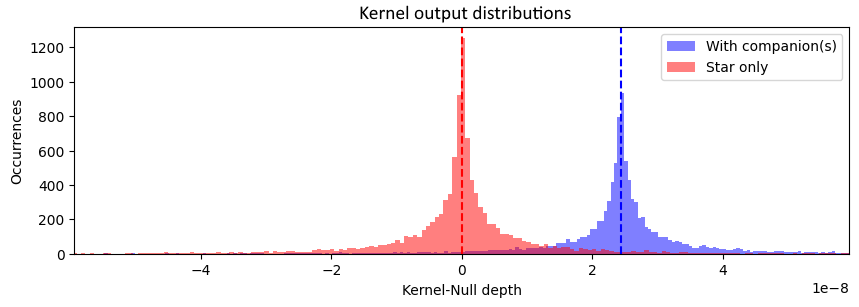
\includegraphics[width=\linewidth]{img/output_distribution.png}
\caption{Example of kernel-null depth distributions for $\mathcal{H}_0$ (star-only) and $\mathcal{H}_1$ (with companion) hypotheses. This example scenario is highly exagerated with a companion that has low contrast in order to induce a significant shift of the distribution. In practice, the two distributions are usually much closer and hard to distinguish.\dm{Cf texte; aussi prends l'habitude d'être ultra-spécifique, c'est un papier scientifique. Là tu es bcp trop vague : "low contrast" (c'est quoi low ?) "much closer" (=?..)}.}
\label{fig:distribution}
\end{figure}

%--------------------------------------------------------------------

\section{Methodology}

\subsection{Data generation}

In this study, we consider two distinct instrumental scenarios for generating simulated data:

\begin{table}[H]
\centering
\begin{tabular}{|l|c|c|}
\hline
\textbf{Parameter} & \textbf{VLTI} & \textbf{LIFE} \\
\hline
Number of telescopes & 4 & 4 \\
Telescope diameter & 8 m & 2 m \\
Configuration & Irregular & Regular (rectangular) \\
Maximum baseline & 130 m & 600 m \\
Operating environment & Ground & Space \\
Wavelength & $1.55\mu$m & $4\mu$m \\
Cophasing error (RMS) & 100 nm & 1 nm \\
\hline
\end{tabular}
\caption{Instrumental parameters for the two scenarios considered in this study.}
\label{tab:scenarios}
\end{table}

The VLTI scenario includes residual cophasing error of 100 nm RMS, representative of atmospheric conditions and phase control system limitations at VLTI. The LIFE scenario benefits from the space environment, allowing a reduction of the cophasing error to 1 nm RMS, reflecting the increased stability expected for a space mission such as LIFE.\dm{Il faut expliquer en détail cette table, que le lecteur ait l'impression de voir les instruments et que tes simus simulent une réalité vraiment réaliste et des manips à portée de main, ça donnera un aspect "chaud" et concret à ton papier.}

For each scenario, datasets are generated under both $\mathcal{H}_0$ (star-only) and $\mathcal{H}_1$ (star-planet system) hypotheses, accounting for specific instrumental parameters and noise levels for each case. The Kernel-Nulling operation is supposed ideal.\dm{Je pense qu'il faut prévoir un appendice où tu résumes le principe de kernel-nulling pour que le lecteur te suive; qu'il comprenne ce que signifie faire une operaiton de kernel nulling en pratique, et lister tous les défauts qui font que ça ne peut pas être idéal. Il faut aussi différencier une operation de kernel null idéale et l'absence de bruit à la fin. Bien expliquer ce que capturent tes simulations et les fluctuations qui créent les distributions montrées en Fig. 1.}

\subsection{Distribution analysis}  \label{sec:distribution_analysis}

Before attempting to discriminate between the $\mathcal{H}_0$ and $\mathcal{H}_1$ hypotheses, it is essential to study the obtained distributions to identify characteristics that might facilitate their analysis. For this purpose, we compare simulated distributions to different conventional probability laws, notably observing their symmetry and general shape.

We find that no conventional law perfectly matches the observed distributions. \dm{$<=$ Ca c'est une conclusion. Pour que cette phrase ait du poids, il faut présenter une analyse détaillée de ces distributions (comme le titre le suggère) : montrer comment les variations combinées de tous les paramètres importants mènent à des distributions différentes. Identifier et montrer tous les différents régimes de paramètres menant à des familles de distributions différentes. Lister aussi tous les pramètres qui vont entrer en compte dans les perfs de détections : contraste et position du compagnon, longueur d'onde donc, nombre de trames, puissance des erreurs de phase, D telescope,... tu peux faire une table. Une étude scientifique est vraiment une étude scientifique : on essaie d'être exhaustif dans l'analyse, et ensuite de faire une synthèse quantifiée et bien rangée qui reflète clairement tous les cas pour le lecteur. Le but est d'en faire un expert en lui donnant toutes les infos pour qu'ils le deviennent en lisant le papier, et puisse reproduire les résultats s'il le souhaite (c'est le propre de la démarche scientifique, éviter d'être juste déclaratif ce qui revient à proposer des arguments d'autorité; préférer systématiquement être aussi précis que possible et donner toutes les infos, ce qui revient à proposer des arguments d'expertise.} Among the tested laws, the Cauchy distribution seems to \dm{c'est faible et pas quantifié, et vu la fig.2 ça ne colle pas comme tu le dis} offer a relatively satisfactory fit (Fig. \ref{fig:fits}), although not perfect, especially on the wings when the number of sample is high.

This observation guides the choice of statistical tests to favor, particularly those effective for detecting shifts in symmetric distributions.\dm{Justifier théoriquement et/ou empiriquement (via l'optique et le ssimus) si les distribution doivent être symétriques. Ajouter éveutellement des acquisitions de frames sur banc pour appuyer à un moment ces hypothèses. } Furthermore, this suggests that data fitting by minimizing \dm{$<=$ data fitting of what ? Pas le fit de d'une distribution empirique par une autre en tout cas... on en discutera. }square error (MSE) will most likely not be very effective due to the heavy tails of the distribution. Instead, we should use a cost function derived from the Cauchy law, which is more robust to outliers:\dm{Non je pense que la fin de la section n'est pas bonne.}
\begin{equation}
    \text{Cost}(x, y) = \sum_i \log \left( 1 + \left( y_i - s(x_i )\right)^2 \right)
\end{equation}

\begin{figure}[H]
\centering
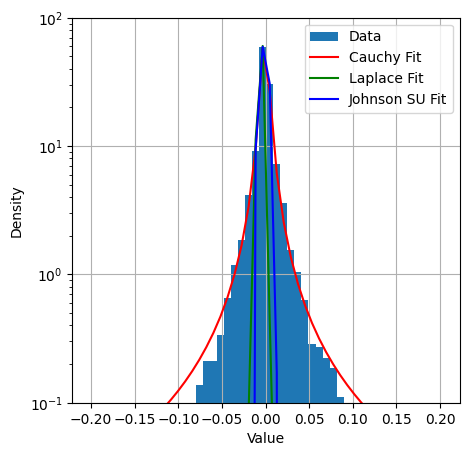
\includegraphics[width=6cm]{img/fits.png}
\caption{Fitting of conventional probability laws to simulated distributions.The Fitter python package was used to perform the fitting of most of the usual laws. This figure show the fit of the three most relevant laws the package pointed out.}
\label{fig:fits}
\end{figure}

\subsection{Statistical tests implemented}

We have developed and compared several test statistics:
\dm{Expliquer la démarche : vu le pb on a logiquement envie d'implémenter  des tests globaux qui mesurent un shift (et rejustifer que c'est juste un shift si c'est bien le cas.\\
- Puis dire qu'on peut aller plus loin : il est naturel de regarder des mesures plus globales entre les distributions et là tu pars sur  KS etc. Ajoute Anderson-Darling dans cette famille.\\
- Ensuite 1) présente tes notations (par ex, qu'est-ce que $x$ ? 2) rappelle précisément ce que tu appelles $\mathcal{H}_0$ et $\mathcal{H}_1$ en utilisant les quantitiés de  tes notations.\\
- Ensuite, pour chaque test, de façon systématique : 0) Donne la ref du/des papiers scientifiques où il a été décrit (pas une ref à une toolbox python; un bouquin tu peux, mais il faut aussi les refs originales \#démarche scientifique vérifiable etc) 1) explique l'intuition derrière 2) donne la stat de test (en utilisant les notations définies avant) 3) explique s'il y a une formule analytique pour décrire la stat de test sous $\mathcal{H}_0$ (explique aussi avant fe lister les tests  que l'intérêt d'une formule analytique est  que ça donne accès à une p-valeur sans avoir à faire des simus de Monte Carlo, et les pbs que posent le fait de devoir faire des MC (calcul mais surtout on doit pouvoir simuler les mêmes conditions de perturbations que les données !)). Par exemple, avec le Th Centrale limite, si les $x_i$ sont i.i.d (pas forcément gaussiens comme dans notre cas), la stat de test (2) est gaussienne de variance connue donc pour (2) ça devrait être bon.\\
- Dans les cas où une distribution est disponible, vérifier par simus et montrer que la distribution empirique correpond bien à la théorique. }
\subsubsection{Mean}

The test statistic based on the mean compares the absolute value of the distribution mean to a threshold:

\begin{equation}
    \left|\frac{1}{N}\sum_i x_i \right| \stackrel{H_1}{\underset{H_0}{\gtrless}} \xi
\end{equation}

\subsubsection{Median}
Test based on the absolute value of the distribution median.

\begin{equation}
\begin{cases}
\left| x_{\frac{N+1}{2}} \right| & \text{if }N\text{ is odd} \\
\left| \frac{x_{\frac{N}{2}} + x_{\frac{N+1}{2}}}{2} \right|  & \text{if }N\text{ is even}
\end{cases}
\quad\stackrel{H_1}{\underset{H_0}{\gtrless}} \xi
\end{equation}

\subsubsection{Argmax}
This statistic examines the position of the bin with the highest number of occurrences in the data histogram.

\hl{Décrire formèlement}

\subsubsection{Kolmogorov-Smirnov}
\dm{Attention c'est le 2-sided KS}
Test comparing the maximum distance between the cumulative distribution functions of the two distributions.

\hl{Décrire formèlement}

\subsubsection{Cramér-von Mises}
Test based on the total quadratic distance between cumulative distribution functions.

\hl{Décrire formèlement}

\subsubsection{Wilcoxon-Mann-Whitney}
Non-parametric test for comparing two independent samples.

\hl{Décrire formèlement}

\subsubsection{CDF difference area}
This statistic measures the area between the cumulative distribution functions of the two distributions.

\hl{Décrire formèlement}

\dm{N'oublie pas le Brunner-Munzel}
%--------------------------------------------------------------------

\dm{Il manque aussi une 3eme approche  ici qui est un GLR : utliser le modèle direct pour calculer la vraisemblance des données selon la position du compagnon; le GLR cherche alors à maximiser la position du compagnon. C'est les formules que j'avais mises au tableau dans mon bureau et la photo est sur discord. On en re-dicte aussi je sais que ça t'avait fait gamberger. C'est important parce que ce test permet la généralisation à plusieurs kernels. \\
D'ailleurs, il faut que tu parles de ça avant de présenter les tests : tu es en seul kernel jusqu'ici. Et il faudra ajouter  une section : Generalisation des tests considérées à plusiers kernels et/ou poses (= comment les stat de tests monokernel-obs peuvent se combiner).}
\section{Results}

\dm{A la fin en bilan fais une lsite des pros et cons de chaque méthode. Il faut que tu déploies dans ce papier une analyse exhaustive et convaincante de la nature des données et des régimes qu'on peut y trouver, des types de distributions suivant les régimes, et des types de tests qu'on peut utiliser. A la fin on se dira que tu as plié le problème, le spécialiste de la détection sur des données kernel-nulling c'est toi !  }
\subsection{ROC curves}

ROC (Receiver Operating Characteristic) curves allow comparing the effectiveness \dm{$<=$ power } of different test statistics by representing the proportion of true detections as a function of false alarm probability.

\begin{figure}[H]
\centering
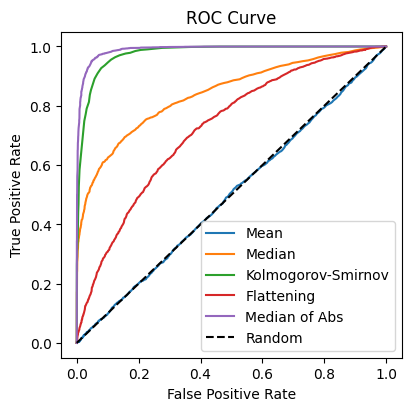
\includegraphics[width=7cm]{img/roc_curves.png}
\caption{ROC curves for different test statistics.}
\label{fig:roc}
\end{figure}

\hl{Analyse des résultats}
\hl{Ajouter la courbe de Neyman-Pearson pour la comparaison}

\subsection{P-value analysis}

\dm{Attention Fig.4 c'est faux : ce ne sont pas les p-valeurs car les p-valeurs ne dépendent pas d'un seuil, seulement des données.}

P-values provide a confidence measure for rejecting the null hypothesis. A P-value below 0.05 is generally considered significant. \dm{Non ça ça dépend des applications. Donne la définition précise de la p-valeur tout de suite, comme ça on sait de quoi on parle. }\\

\dm{Pour l'approche Neyman-Pearson (ou Likelihood-Ratio), il faut en faire une section à part dans la section d'avant en explicitant le Likelihood-Ratio et les paramètres dont il dépend sous les 2 hypothèses, puis en tirer la stat de test que ça donne en prenant le log etc .\\
Expliquer aussi l'intérêt du NP.}.


\begin{figure}[H]
\centering
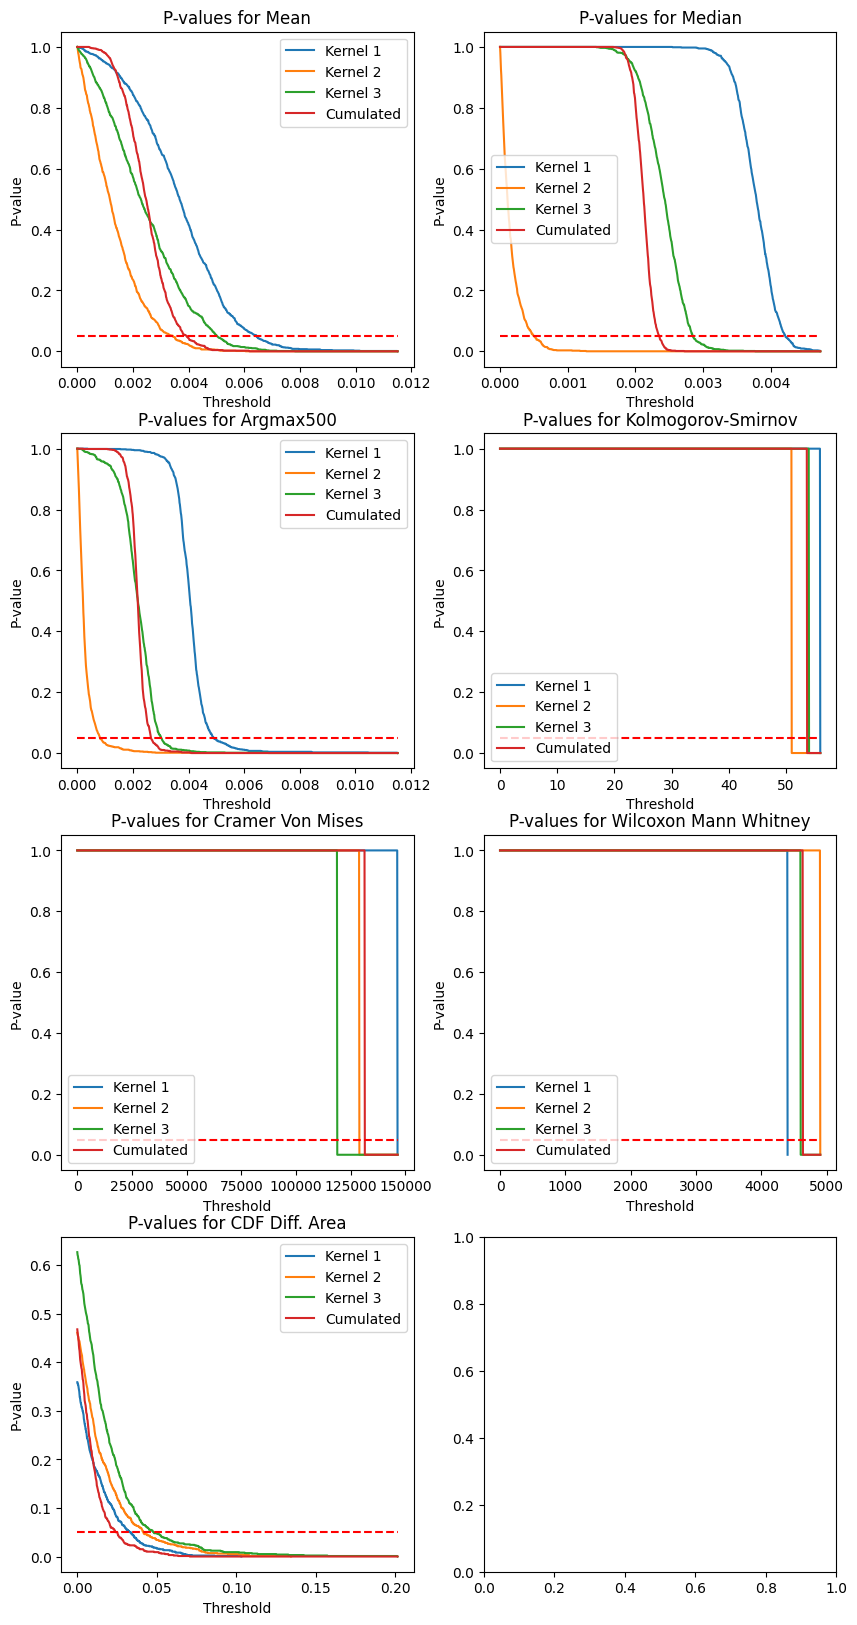
\includegraphics[width=10cm]{img/p-values.png}
\caption{Evolution of P-values as a function of threshold for different test statistics. The red dotted line indicates the significance threshold at 0.05. \hl{Plot à refaire pour se focaliser sur un seul Kernel (+ correction des bugs)} \dm{Oui. On peut par exemple montrer la calibration théorique p-valeur(stat de test - pas seuil !) et comparer à la calibration empirique pour chaque test }}


\label{fig:pvalues}
\end{figure}

\hl{Analyse des résultats}

%--------------------------------------------------------------------

\section{Discussion}

\subsection{Comparative test performance}

\hl{ToDo}

\subsection{Noise sensitivity}

\hl{ToDo}


%-----------------------------------------------------------------

\section{Conclusions}

\hl{ToDo}

\bibliographystyle{alpha}
\bibliography{sample}

\end{document}